%*****************************************
\chapter{Data Dispersion} \label{dis:data_dispersion}
%*****************************************
%TODO Reviewed

\section{Introduction}

One way to describe a dataset is to report its dispersion, or spread. For example, if a professor administered a test to $ 100 $ students and the scores were between $ 90 - 100 $ that would be a fairly tight group but if another class had scores between $ 60 - 100 $ that would indicate something completely different. This lab explores the concept of data dispersion and the methods used to describe that value.

\section{Measures of Data Dispersion}

\subsection{Range}

The maximum and minimum values are those at the extreme ends of the dataset and the range is nothing more than the maximum minus the minimum values. For the $ 2016 $ version of the Scholastic Aptitude Test (SAT) the maximum score is $ 1600 $ and the minimum score is $ 400 $, so the range is $ 1600-400 $, or $ 1200 $.

\subsection{Quartiles}

A measure that is closely related to the median\footnote{The median was described in Lab \ref{cen:median}, page \pageref{cen:median}.} is the first and third quartile. The first quartile (\textit{Q1}) is the score that splits the lowest $ 25\% $ of the values from the rest and the third quartile (\textit{Q3}) splits the highest $ 25\% $ of the values from the rest. The second quartile (\textit{Q2}) is the same as the median and, normally, the term ``median'' is used rather than \textit{Q2}. For example, consider this dataset: 

\begin{center}
  $ 5, 7, 10, 13, 17, 19, 23 $
\end{center}

The median of this dataset is $ 13 $ because three values are smaller and three are larger. The first quartile is $ 7 $, which is the median for the lower half of the values (not including $ 13 $, the median of the dataset); or the score that splits the lowest $ 25 \% $ from the rest of the data. The third quartile is $ 19 $, which is the median for the upper half of the scores; or the score that splits the highest $ 25 \% $ from the rest of the data. 

Occasionally, the word ``hinges'' appears in statistical literature. The two hinges for a dataset are the medians for the lower half and the upper half of the data, but those halves also include the dataset median. For the simple dataset above, the lower hinge is the median of $ 5 $, $ 7 $, $ 10 $, and $ 13 $, or $ 8.5 $. The upper hinge is the median of $ 13 $, $ 17 $, $ 19 $, and $ 23 $, or $ 18 $. Quartiles and hinges usually have about the same accuracy but quartiles are more commonly used.

Another measure of dispersion that is occasionally used is the Inter-Quartile Range (\textit{IQR}); that is, the difference between \textit{Q1} and \textit{Q3}. This is used to counter the skew introduced by a dataset with extreme outliers.

\subsection{Standard Deviation}\label{dis:standard_deviation}

The standard deviation of a dataset is a number that indicates how much variation there is in the data; or how ``scattered'' the data are from the mean. In general, the larger the standard deviation then the more variation there is in the data. A dataset with a small standard deviation would create a sharply peaked normal distribution curve while a large standard deviation would create a flatter curve.\footnote{The concept of the normal distribution curve was presented in Lab \ref{int:normal_distribution} on page \pageref{int:normal_distribution}.}

Once a standard deviation is calculated, then about $ 68.2 $\% of the samples will lie closer to the mean than that number. To put it another way, one standard deviation explains about $ 68.2 $\% of the variance from the mean. To show this concept graphically, consider the following graph of the scores on an examination:

\begin{figure}[H]
  \begin{center}
    \fbox{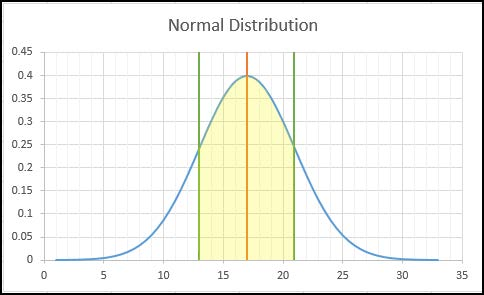
\includegraphics[width=\linewidth]{gfx/dis005}}
    \caption{Illustration Of Standard Deviation}
  \end{center}
\end{figure}

The mean of this distribution is marked with a vertical line in the center of the bell curve. One standard deviation up and one standard deviation down are marked by two other vertical lines. The shaded area under the curve would include about $ 68.2 $\% of all scores for this dataset. In the same way, two standard deviations from the mean would include about $ 95.4 $\% of the data points; and three standard deviations would include more than $ 99.7 $\% of the data points (these larger values are not indicated on the graph).

As one last example, imagine a class with $ 500 $ students where the professor administered an examination worth $ 100 $ points. If the mean score for that examination was $ 80 $ and the standard deviation was $ 5 $, then the professor would know that the scores were fairly tightly grouped ($ 341 $ scores of the $ 500 $ ($ 68.2 $\%) were between $ 75-85 $, within $ 5 $ points of the mean), and this would probably be good news for the professor. On the other hand, if the mean score was $ 60 $ and the standard deviation was $ 15 $, then the scores were ``all over the place' (more precisely, $ 341 $ scores of the $ 500 $ were between $ 45 $-$ 75 $), and that may mean that the professor would have to re-think how the lesson that was taught or that the examination itself was flawed.

It is difficult to categorically state whether a specific standard deviation is good or bad; it is simply a measure of how concentrated the data are around the mean. For something like a manufacturing process where the required tolerance for the parts being produced is tight then the standard deviation for the weights of random samples pulled off of the line must be very small; that is, the parts must be as nearly identical as possible. However, in another context, the standard deviation may be quite large. Imagine measuring the time it takes a group of high school students to run $ 100 $ yards. Some would be very fast but others would be much slower and the standard deviation for that data would likely be large. 

\section{Procedure}

\subsection{Statistical Calculations}
\label{dis:statistical_calculations}

Start \texttt{SOFA} and select ``Report Tables.'' Then:

\begin{enumerate}
  \item Data Source Table: dbims
  \item Table Type: Row Stats
  \item Columns: Age (age)
  \item Title: Age Statistics
  
  \begin{figure}[H]
      \begin{center}
          \fbox{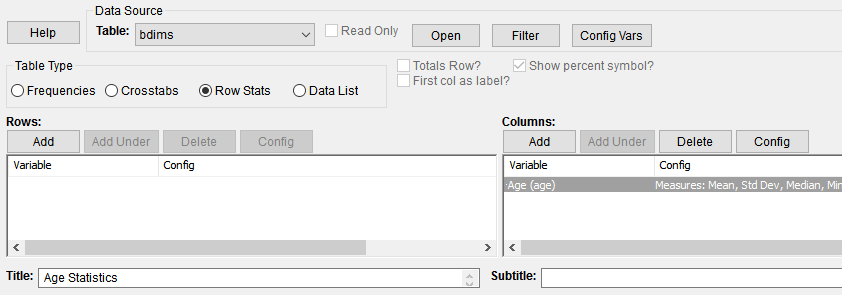
\includegraphics[width=0.90\linewidth]{gfx/dis010}}
          \caption{Setting Up Age}
        \end{center}
  \end{figure}
    
  \item Just above the ``Columns'' window, click the ``Config'' button and select: Mean, Standard Deviation, Median, Minimum, and Maximum. Of course, any of the available measures, such as range or quartiles, can be selected depending upon what needs to be reported.
    
  \begin{figure}[H]
      \begin{center}
          \fbox{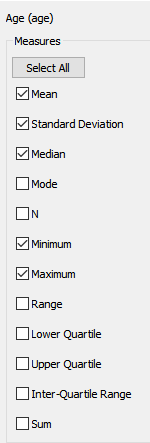
\includegraphics[]{gfx/dis015}}
          \caption{Configure Options for Age}
      \end{center}
  \end{figure}
    
  \item Read those values in the lower left corner of the ``Make Report Table'' window.

  \begin{figure}[H]
    \begin{center}
      \fbox{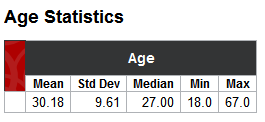
\includegraphics[]{gfx/dis020}}
      \caption{Statistics for Age}
    \end{center}
  \end{figure}
  
\end{enumerate}

\subsection{Activity 1: Simple Statistics} \label{dis:act01}

Using the \textit{maincafe} dataset in \texttt{SOFA}, produce a table that contains the standard deviation, minimum, maximum, range, lower quartile, upper quartile, and inter-quartile range for Age. The table should have a title of ``Data Dispersion, Activity 1'' and a subtitle of ``Measures of Dispersion''.

\subsection{Grouping Variables}

To produce the statistics for grouped variables, like ``the age statistics by sex,'' add the ``sex'' variable to the ``Rows:'' window and modify the title of the chart.

\begin{figure}[H]
  \begin{center}
    \fbox{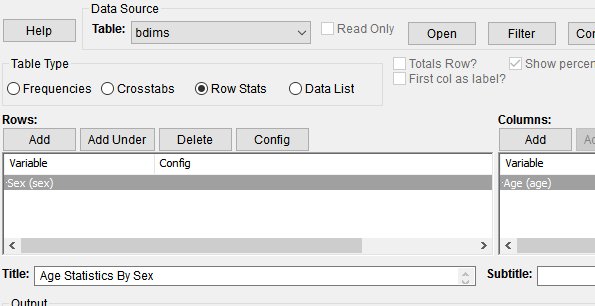
\includegraphics[width=\linewidth]{gfx/dis025}}
    \caption{Grouping Age Statistics by Sex}
  \end{center}
\end{figure}
 
Then, the output will display the selected Age statistics by sex.

\begin{figure}[H]
  \begin{center}
    \fbox{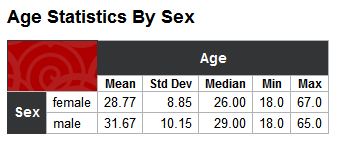
\includegraphics[]{gfx/dis030}}
    \caption{Age Statistics by Sex}
  \end{center}
\end{figure}

\subsection{Activity 2: Grouped Statistics} \label{dis:act02}

Using the \textit{maincafe} dataset in \texttt{SOFA}, produce a table that contains the mean, standard deviation, and N for Age when grouped by Sex. The table should have a title of ``Data Dispersion, Activity 2'' and a subtitle of ``Grouped Measures of Dispersion''.

\subsection{Filtering}

\texttt{SOFA} provides researchers a way to filter the data such that only a specified subset is used in calculations. As an example, to analyze only the males in the dataset:

Start \texttt{SOFA} and select ``Report Tables.'' Then:

\begin{enumerate}
  \item Data Source Table: dbims
  \item Table Type: Row Stats
  \item Columns: Age (age)
  \item Configure the Age column to display the Mean, Median, and N
  \item Title: Age Statistics For Males
  \item Click the ``Filter'' button near the top of the window
  \item Select ``Sex'' in the dropdown list for the ``Quick'' button
  \item Select the ``$ = $'' comparator
  \item Enter ``male'' as the match term (Note: do not use quote marks)
  \item Add the optional label: ``Analyze Age For Males Only''
\end{enumerate}
  
\begin{figure}[H]
  \begin{center}
    \fbox{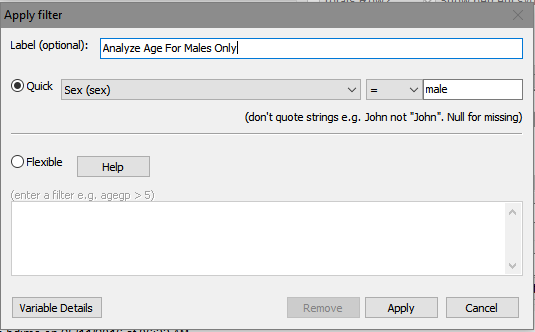
\includegraphics[width=\linewidth]{gfx/dis035}}
    \caption{Setting Up a Filter}
  \end{center}
\end{figure}

Then, the output will display the selected Age statistics for males only.

\begin{figure}[H]
  \begin{center}
    \fbox{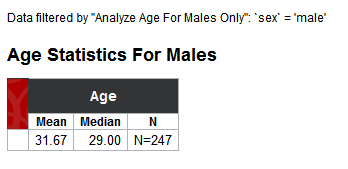
\includegraphics[]{gfx/dis040}}
    \caption{Age Statistics for Males}
  \end{center}
\end{figure}

\textbf{Important Note: Once a filter is applied it will remain until it is either manually removed or the \texttt{SOFA} session ends.} To remove a filter, open the filter dialog box and click the ``remove'' button.

\subsection{Activity 3: Filtering} \label{dis:act03}

Using the \textit{maincafe} dataset in \texttt{SOFA}, produce a table that contains the mean, standard deviation, and N for Age for only males. The table should have a title of ``Data Dispersion, Activity 3'' and a subtitle of ``Filtered Statistics''.

\section{Deliverable}

Complete the following activities in this lab:

\rowcolors{1}{gray!25}{}
\begin{center}
  \begin{tabular}{lll}
    \hline 
    \textbf{Number} & \textbf{Name} & \textbf{Page} \\ 
    \hline 
    \ref{dis:act01} & \nameref{dis:act01} & \pageref{dis:act01} \\ 
    \ref{dis:act02} & \nameref{dis:act02} & \pageref{dis:act02} \\ 
    \ref{dis:act03} & \nameref{dis:act03} & \pageref{dis:act03} \\ 
    \hline 
  \end{tabular} 
\end{center}

Consolidate the responses for all activities into a single document and submit that document for grading.
